%% Reliability-Targeted Model Inversion with Explicit Infeasibility
%% IEEE AAIML 2027 (2nd Int. Conf. on Advances in AI and Machine Learning),
%% Nihon University, Tokyo, 29-31 March 2027.
%%
%% Confirmed against https://www.aaiml.net/sub.html on 2026-10-01:
%%   Deadline   10 Oct 2026      Notify  10 Nov 2026
%%   Limit      6 pages; up to 4 extra at USD 70/page; 10 pages absolute max
%%   Review     DOUBLE-BLIND, submissions must be anonymised, and authors'
%%              own prior work may not be cited in an identifying way
%%   System     EasyChair (easychair.org/conferences/?conf=aaiml2027)
%%   Output     IEEE Xplore, submitted to Scopus and Ei Compendex
%%   Originality: "must be original and not simultaneously submitted to
%%              another journal or conference"
%%
%% Fit: Track 1 "Innovations in Machine Learning Algorithms" (Explainable AI),
%% secondarily Track 3 "Applications ... Across Industries" (Healthcare).
%%
%% Build:  pdflatex aaiml2027 && pdflatex aaiml2027
%% Figures live in figures/ ; regenerate with
%%   python evaluation/run_study.py --figures figures/

\documentclass[conference]{IEEEtran}
\IEEEoverridecommandlockouts

\usepackage{cite}
\usepackage{amsmath,amssymb}
\usepackage{graphicx}
\usepackage{booktabs}
\usepackage{algorithm}
\usepackage{algpseudocode}
\usepackage{url}
\usepackage[T1]{fontenc}

\graphicspath{{figures/}}

% Six pages is the free limit, so floats are kept tight.
\setlength{\textfloatsep}{7pt plus 2pt minus 2pt}
\setlength{\floatsep}{7pt plus 2pt minus 2pt}
\setlength{\intextsep}{7pt plus 2pt minus 2pt}

%% Double-blind: pdfTeX otherwise writes the system username into /Author.
\ifdefined\pdfinfo
  \pdfinfo{%
    /Author ()%
    /Title (Reliability-Targeted Model Inversion with Explicit Infeasibility)%
    /Subject ()%
    /Keywords ()%
    /Creator ()%
  }
\fi

\begin{document}

\title{Reliability-Targeted Model Inversion\\with Explicit Infeasibility}

%% ---------------------------------------------------------------
%% AAIML 2027 is DOUBLE-BLIND. Leave \anontrue for the 10 Oct submission.
%% Flip to \anonfalse only for camera-ready, and for any preprint posted
%% after the submission goes in. The real block lives in authors.local.tex,
%% which is gitignored so no name exists anywhere in the repository.
%% ---------------------------------------------------------------
\newif\ifanon
\anontrue                        % <<< \anonfalse for camera-ready

\ifanon
  \author{\IEEEauthorblockN{Anonymous Authors}
  \IEEEauthorblockA{Affiliation withheld for double-blind review}}
\else
  \IfFileExists{authors.local.tex}{\input{authors.local.tex}}{%
    \PackageError{aaiml2027}{authors.local.tex is missing}{%
      Camera-ready needs paper/authors.local.tex (gitignored, so it is not in
      a fresh clone). Recreate it with the \string\author{} block, or set
      \string\anontrue to build the anonymous version.}}
\fi

\maketitle

\begin{abstract}
Algorithmic recourse asks what a person must change to flip a decision a model
has already made about them. We study the related problem in which the
constraint is a probability the user chooses rather than a label the model
assigns, and in which the search space is bounded by time. Our method inverts a
trained classifier against a required reliability, searching only over inputs
the user can act on within the planning horizon, and it returns an explicit
infeasibility verdict with counterfactual attribution whenever no admissible
change reaches the target. The horizon partition is the part we claim as new.
Recourse separates inputs into actionable and immutable, but many real inputs
are neither, being entirely changeable over weeks and unavailable today, and
treating them either way produces advice that cannot be followed or discards the
best available explanation of why the target is out of reach. Validated against
exhaustive search over seven ground-truth models, the method never promises an
unreachable target, it returns the optimal admissible point in every case, and
it selects a minimal change set, so its only failure mode is conservatism. An
ablation shows the horizon partition is the sole component whose removal makes
the method promise what cannot be delivered. We evaluate on a sleep planning
task over two public wearable cohorts covering 85 participants and 5,432
person-nights, where the underlying models are weak, reaching an $R^2$ of 0.186
for sleep duration and an AUC of 0.660 for wake-time regularity while remaining
well calibrated at an expected calibration error of 0.0148. We also find that a
physiologically structured synthetic panel overstates predictability on the same
task by roughly fourfold in $R^2$, which matters because training on simulated
data is common. Weak models motivate the contribution rather than undermining
it, since a system working from a signal this thin should be able to decline.
\end{abstract}

\begin{IEEEkeywords}
explainable AI, algorithmic recourse, counterfactual explanation, model
inversion, actionability, calibration, constrained search, wearable sensing
\end{IEEEkeywords}

%% ===============================================================
\section{Introduction}

A trained classifier is normally read forward. Features go in, a probability
comes out, and the user is left to work out what to do about it. Counterfactual
explanation and algorithmic recourse read the same model backwards instead,
asking what minimal change to the input would flip the decision, and that
reframing is what turns a prediction into advice.

Two assumptions in that literature do not survive contact with planning
problems. The first is that the thing being searched for is a label. Recourse
flips a decision the model has made about a person, such as a loan denial. But a
user who must meet an obligation does not want a label flipped, they want a
stated level of confidence, and the difference between wanting the decision
changed and wanting an eighty-five percent chance of an outcome is the
difference between crossing a boundary and satisfying a threshold.

The second is that inputs divide into actionable and immutable. Age is
immutable, income is actionable, and the search runs over the second set. Many
real inputs sit in neither class. Habits are entirely changeable, over weeks,
and completely unavailable within the horizon the user is planning over.
Treating them as actionable yields advice nobody can follow tonight. Treating
them as immutable throws away the most useful thing the model can say when the
target cannot be reached, which is that the obstacle is a habit rather than
anything about today.

We make three contributions.

\textbf{Reliability-targeted inversion.} We solve for the least costly
admissible input that attains a user-specified probability, rather than the
nearest input across a decision boundary.

\textbf{A partition by planning horizon.} Inputs are divided by when the user
can act on them rather than by whether they can act on them at all. Our ablation
shows this is the only component whose removal causes the method to recommend
changes that cannot be made in time.

\textbf{Infeasibility as a first-class output.} When no admissible change
reaches the target, the method says so, reports the attainable ceiling, and
attributes the shortfall to the specific out-of-horizon input responsible. We
argue this matters most when models are weak, and we show on real data that
models in our domain are weak.

Section~\ref{sec:related} positions the work against recourse and counterfactual
explanation. Section~\ref{sec:method} specifies the method.
Section~\ref{sec:results} validates the search against exhaustive ground truth,
ablates it, and reports what happens on two public cohorts.
Sections~\ref{sec:limitations} and~\ref{sec:conclusion} state what the evidence
does not support.

%% ===============================================================
\section{Related Work}
\label{sec:related}

The closest technical neighbours are counterfactual explanation~\cite{wachter}
and algorithmic recourse~\cite{ustun,dice}. Wachter et al.~\cite{wachter}
generate the minimal input change that flips a model's decision.
DiCE~\cite{dice} extends this to diverse sets of such changes. Ustun et
al.~\cite{ustun} are nearest of all, separating \emph{actionable} inputs from
\emph{immutable} ones and searching only over the former, on the grounds that
recourse offered over age or marital status is no recourse at all.

We differ in three ways, and the third is the one we claim as novel.

\textbf{The constraint is a probability, not a label.} Recourse asks what flips
a decision already made about a person. We ask what attains a stated probability
of a future outcome the person chose for themselves. The target is a continuous
threshold on $f$ rather than a decision boundary, and the objective is the least
costly point satisfying it rather than the nearest point across it.

\textbf{The partition is temporal, not binary.} Recourse divides inputs into
actionable and immutable. A third class fits neither label, being entirely
changeable over a longer horizon and unavailable within the one the user is
planning over. We therefore partition by planning horizon rather than by
mutability, and Section~\ref{sec:ablation} shows this is the only component
whose removal causes the method to promise what cannot be delivered.

\textbf{Infeasibility is an output, not a failure.} When no recourse exists,
recourse methods report that none was found. We treat that case as a primary
result, reporting the attainable ceiling and attributing the shortfall by
counterfactual substitution over the out-of-horizon inputs, which converts ``no
plan exists'' into ``the limit is not today, it is this habit, worth this much.''
For a user who must not fail, that is more actionable than a plan would be.

Our evaluation domain has its own forward literature. Sleep outcomes are widely
predicted from wearable data, from deep models of sleep
quality~\cite{sathya} to next-night duration in clinical
populations~\cite{fellger}, and consumer smart alarms optimise \emph{when to
ring inside a given window}~\cite{smartalarm}, which is a different problem from
solving for the behaviour that precedes a fixed deadline. All of that work runs
forward. Our contribution is not a better predictor, ours is weak and we report
it as such, but a way of using a predictor that stays honest when it is weak.

%% ===============================================================
\section{Method}
\label{sec:method}

\subsection{Problem formulation}

Let $\mathbf{x} \in \mathbb{R}^d$ be a feature vector and
$f(\mathbf{x}) \rightarrow [0,1]$ a trained classifier estimating the
probability of a desired outcome. A forward system reports $f(\mathbf{x})$. We
instead solve, for a required reliability $\tau$: find the least costly
admissible $\mathbf{x}'$ such that $f(\mathbf{x}') \ge \tau$, and if none
exists, report that fact together with the attainable ceiling and its cause.

In our instantiation the primary control is a continuous scheduling variable and
least costly means latest, since among settings that satisfy the constraint the
latest imposes the smallest behavioural change. This is a design choice with a
trade-off rather than an obvious optimum. The latest feasible point is by
construction the one with no margin, sitting exactly at the constraint boundary,
so any error in $f$ translates directly into a failed outcome. The objective is
therefore exposed as a parameter, so a deployment can require
$f \ge \tau + m$ for a margin $m$, and we make no claim that $m = 0$ is right
for users.

\subsection{The horizon partition}

The $d$ inputs are divided into three classes, and only the first is admissible
in a within-horizon plan. \textbf{Controllable now} holds the inputs the user
can set today, which in our instantiation are bedtime, pre-sleep screen time,
caffeine, ambient noise, room temperature, stress and exercise.
\textbf{Out-of-horizon} holds inputs that are genuinely changeable but only over
weeks, namely sleep-timing consistency, habitual snooze count, habitual alarm
response latency and accumulated sleep debt. \textbf{Fixed} holds age,
chronotype and resting heart rate.

This is the distinction recourse does not draw. The middle class is not
immutable, and a method that labels it so loses the ability to explain a
refusal, while a method that labels it actionable produces plans that cannot be
executed in time.

\textbf{The middle class is not peculiar to sleep.} It appears wherever an input
is an accumulated summary of past behaviour, which is common in exactly the
domains recourse is usually demonstrated on. In credit, an applicant can pay
down a balance today, but length of credit history and depth of payment history
move only over months, so advice to improve them is correct and useless when the
decision is tomorrow. In clinical decision support, a patient can change today's
diet and adherence, while HbA1c summarises roughly three months of glycaemic
control and cannot be moved by the next appointment. In both cases a binary
split mislabels the summary input, and the choice of which way to mislabel it
determines whether the system produces unachievable advice or silently drops the
best explanation it has. Partitioning by horizon makes the distinction explicit
and lets the same model serve a user planning for tomorrow and a user planning
for next quarter, by changing which partition is admissible rather than
retraining.

\subsection{Inverse search}

\begin{algorithm}[t]
\caption{Primary-control sweep}
\label{alg:sweep}
\begin{algorithmic}[1]
\Require features $\mathbf{x}$, target $\tau$
\Ensure optimal admissible value or $\perp$, ceiling, full curve
\State $B \gets$ admissible range, ordered least-costly first
\State $S \gets f_{\text{batch}}(\{\mathbf{x}\ \text{with control}\ b : b \in B\})$
\State $\textit{best} \gets \max(S)$
\ForAll{$(b, s) \in \text{zip}(B, S)$}
  \If{$s \ge \tau$} \Return $b$, \textit{best}, curve \Comment{first hit is optimal}
  \EndIf
\EndFor
\State \Return $\perp$, \textit{best}, curve
\end{algorithmic}
\end{algorithm}

\textbf{Algorithm~\ref{alg:sweep}} sweeps the primary control across its
admissible range at fixed resolution, scores all candidates in one batched
forward pass, and returns the least costly candidate meeting $\tau$. In our
instantiation that is 25 bedtimes spanning 20:00 to 02:00 at 15-minute steps.

Exhaustive scanning rather than gradient search is deliberate. A random forest's
response is a step function with no gradient to follow, the admissible range is
narrow, and the whole curve is worth returning for display.
Section~\ref{sec:sound} confirms the sweep returns the true optimum in every
simulated scenario including non-monotone response curves, where a gradient
method would settle in a local optimum.

\begin{algorithm}[t]
\caption{Greedy coordinate ascent over remaining controls}
\label{alg:ascent}
\begin{algorithmic}[1]
\Require features $\mathbf{x}$, target $\tau$, budget $R$
\Ensure modified features, attained reliability, change set
\State $c \gets \mathbf{x}$;\ \ $r \gets f(c)$;\ \ \textit{steps} $\gets [\,]$
\For{$R$ rounds}
  \If{$r \ge \tau$} \textbf{break} \EndIf
  \State $M \gets \{\text{clamp}(v + \text{dir}\cdot\text{step}\cdot 3)\}$ per control
  \State $M \gets \{m \in M : m\ \text{changes the current value}\}$
  \If{$M = \emptyset$} \textbf{break} \EndIf
  \State $G \gets f_{\text{batch}}(\{c \oplus m : m \in M\})$
  \State $i \gets \arg\max(G)$;\ \ \textit{gain} $\gets G[i] - r$
  \If{\textit{gain} $\le 0.002$} \textbf{break} \EndIf
  \State merge $M[i]$ into \textit{steps} \Comment{fold repeats on one control}
  \State $c \gets c \oplus M[i]$;\ \ $r \gets G[i]$
\EndFor
\State \Return $c$, $f(c)$, \textit{steps}
\end{algorithmic}
\end{algorithm}

\textbf{Algorithm~\ref{alg:ascent}} searches the remaining controllable inputs
one at a time when the primary control alone is insufficient. Two details matter
for reimplementation. Re-scoring after each committed move is what prevents
double-counting redundant inputs, because two controls acting through one
underlying channel do not contribute additively and scoring them independently
overstates the plan. Stopping as soon as $\tau$ is met yields the fewest changes
that suffice rather than every change available, and
Section~\ref{sec:sound} confirms the resulting set is exactly minimal.

We set $R = 8$. It was 3 until simulation showed the search exhausting its
budget rather than its options, with a traced case reaching 0.66 against a 0.70
target and needing one further round. Raising it cut false refusals from 10 to 3
of 42 and never once produced an unkeepable promise. Each round moves the chosen
control by three steps of its native resolution, and a move is committed only if
it gains at least 0.002.

Table~\ref{tab:levers} gives the instantiation in full, since a search method is
only reproducible if the admissible set is stated. Room temperature is the one
control with no monotone direction, so its candidate is a set-point rather than
an extreme, because both hotter and colder are worse. The out-of-horizon inputs
are counterfactually set to sleep consistency 85/100, zero snoozes, a 5{,}000\,ms
alarm response and zero sleep debt when attributing a refusal.

\begin{table}[t]
\caption{The admissible set and the search thresholds}
\label{tab:levers}
\centering
\small
\begin{tabular}{lccc}
\toprule
Control & Dir. & Range & Step \\
\midrule
\texttt{bedtime\_hour}                & $-$ & 20.0--26.0\,h & 0.25 \\
\texttt{screen\_minutes\_before\_bed} & $-$ & 0--180\,min & 15 \\
\texttt{caffeine\_mg}                 & $-$ & 0--400\,mg & 40 \\
\texttt{ambient\_noise\_db}           & $-$ & 20--70\,dB & 5 \\
\texttt{room\_temp\_c}        & set-pt. & 14--30\,\textdegree C & $\rightarrow$ 20.5 \\
\texttt{stress\_level}                & $-$ & 0--100 & 10 \\
\texttt{exercise\_minutes}            & $+$ & 0--120\,min & 20 \\
\midrule
\multicolumn{4}{l}{\emph{Thresholds}}\\
Coordinate-ascent budget $R$      & \multicolumn{3}{c}{8 rounds} \\
Min.\ gain to commit a move       & \multicolumn{3}{c}{0.002} \\
Min.\ gain to report a control    & \multicolumn{3}{c}{0.001} \\
Min.\ gain to report a cause      & \multicolumn{3}{c}{0.01} \\
Primary-control resolution        & \multicolumn{3}{c}{0.25\,h over 20:00--02:00} \\
\bottomrule
\end{tabular}
\end{table}

\subsection{Infeasibility and attribution}

If neither algorithm reaches $\tau$, the method returns no plan. It returns the
attainable ceiling and attributes the shortfall to the out-of-horizon partition
by counterfactual substitution, setting each such input independently to a
healthy reference value, re-scoring, and reporting those yielding a gain above
0.01, ranked, with the horizon on which they could be changed.

The output takes the form \emph{``95\% is not reachable today, the best
available combination reaches 60\%, and what limits you is habit rather than
anything about today: responding to your alarm on the first attempt is worth 30
points on its own.''} Fig.~\ref{fig:search} contrasts the two cases the method
distinguishes.

\begin{figure}[t]
\centering
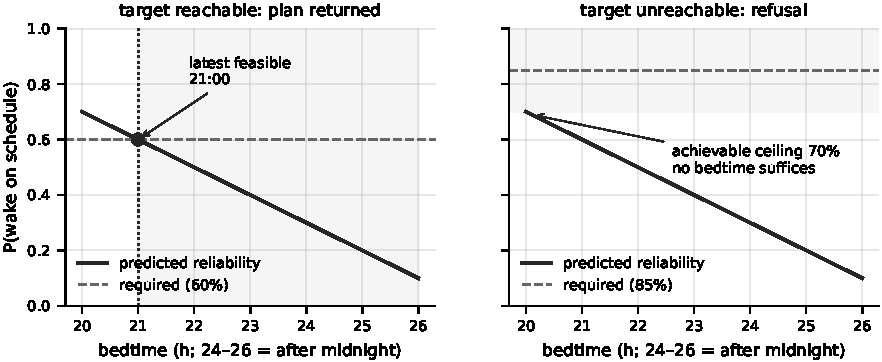
\includegraphics[width=\columnwidth]{fig1_inverse_search.pdf}
\caption{Inverse search on a feasible instance (left) and an infeasible one
(right). The sweep returns the least costly setting clearing $\tau$. Where the
whole curve sits below $\tau$, the method refuses and reports the ceiling
instead of a plan.}
\label{fig:search}
\end{figure}

\subsection{Experimental setup}

\textbf{Simulation.} The search is validated against exhaustive search over
seven analytic ground-truth models crossed with six targets, giving 42
scenarios. The models were written to defeat greedy search rather than to
flatter it, and include non-monotone response curves, redundant controls,
interacting controls and hard ceilings.

\textbf{Cohorts.} The real-data evaluation uses two public wearable datasets
that require no application, LifeSnaps~\cite{lifesnaps} (69 participants with
sleep data, 3,551 person-nights, Fitbit Sense) and PMData~\cite{pmdata} (16
participants, 1,881 person-nights, Fitbit Versa 2). Feature availability is the
binding constraint. Of 15 model inputs only 3 to 4 are directly available and 5
derivable, and no public wearable dataset records alarm interaction, so two of
the four out-of-horizon inputs cannot be populated at all.

\textbf{Target.} Neither dataset contains an alarm, so the outcome is
constructed. A night is labelled successful when the participant woke no more
than 30 minutes after their habitual wake time for that type of day, computed
within participant and day-type over a 28-night trailing window using prior
nights only. We call this \emph{wake-time regularity} rather than wake success,
for the reason given in Section~\ref{sec:limitations}. A sweep over the three
construction choices shows tolerance is robust, with labels agreeing 0.923 when
halved to 15 minutes and 0.886 when doubled to 60, and day-type bucketing nearly
free in aggregate at a positive-rate spread of 0.040 while still flipping 16\%
of nights against a pooled baseline. One-sidedness is the consequential choice,
flipping a quarter of nights.

\textbf{Models and protocol.} Random forests (200 trees, depth 12, minimum leaf
8, seed 42) for both a duration regressor and a regularity classifier, matching
the configuration used on a synthetic panel so that differences isolate the
data. Splits are by participant over 8 grouped splits, since splitting rows at
random lets a model identify the person rather than learn about nights. Outcome
columns are excluded from the features by assertion rather than convention, and
trailing features use strictly prior nights, since including the current value
leaks the target. All intervals come from resampling participants rather than
rows. Complete cases only, which leaves 3,376 nights from 63 participants on
LifeSnaps.

%% ===============================================================
\section{Results}
\label{sec:results}

\subsection{The search is sound but incomplete}
\label{sec:sound}

The recommendation itself cannot be validated observationally, because it is
conditional on a setting no participant adopted on our instruction. We therefore
validate the \emph{algorithm} against exhaustive search over the 42 scenarios
(Table~\ref{tab:sound}).

\begin{table}[t]
\caption{Validation against exhaustive search over 42 scenarios}
\label{tab:sound}
\centering
\small
\begin{tabular}{lc}
\toprule
Property & Result \\
\midrule
Sweep returns the optimal admissible setting & $\mathbf{42/42}$ \\
Promises only reachable targets (soundness) & \textbf{0 violations} \\
Change set exactly minimal when successful & 100\% \\
Refuses only unreachable targets (completeness) & 92.9\% (3/42) \\
\bottomrule
\end{tabular}
\end{table}

The method never over-promises at any iteration budget tested. Its failure mode
is conservatism, refusing three targets that were in fact achievable, which for
a system whose contribution is honest refusal is the correct direction to err.
Behaviour at the attainable ceiling is exact, in that a target equal to the
ceiling is promised and one 0.001 above it is refused.

\subsection{The horizon partition is the load-bearing component}
\label{sec:ablation}

Table~\ref{tab:ablation} removes each component in turn. The sweep buys
optimality rather than feasibility, and without it minimality falls from 1.00 to
0.56. Coordinate ascent buys completeness, and without it false refusals more
than triple. Attribution changes no verdict at all, only whether the user is
told why.

\begin{table}[t]
\caption{Ablations. Only removing the horizon partition breaks soundness.}
\label{tab:ablation}
\centering
\small
\begin{tabular}{lcccc}
\toprule
Ablation & Verdict & False & Broken & Optimal \\
 & correct & refusals & promises & setting \\
\midrule
Full method & 0.929 & 3 & \textbf{0} & 1.00 \\
No sweep & 0.881 & 5 & 0 & \textbf{0.69} \\
No coordinate ascent & \textbf{0.762} & \textbf{10} & 0 & 1.00 \\
No horizon partition & 0.857 & 3 & \textbf{3} & 1.00 \\
No attribution & 0.929 & 3 & 0 & 1.00 \\
\bottomrule
\end{tabular}
\end{table}

\textbf{Only removing the horizon partition breaks soundness.} Without it the
method offers plans requiring changes that cannot be made within the horizon, so
it promises outcomes the world cannot deliver. This is the result that justifies
treating the partition as a contribution rather than an implementation detail.

It is also the paper's least externally grounded claim, and the two facts are
connected. The partition is exercised here only in simulation, and two of its
four inputs do not exist in any public wearable dataset, so no observational
analysis we can run tests it. We take the simulation as evidence that the
mechanism works as designed, not as evidence that it is calibrated to human
behaviour.

\subsection{Synthetic data substantially overstates predictability}

Our own system was developed against a physiologically structured synthetic
panel before real cohorts were obtained. Retraining with identical model,
features and protocol on real data (Table~\ref{tab:synthgap},
Fig.~\ref{fig:synthgap}) drops $R^2$ by roughly a factor of four.

\begin{table}[t]
\caption{Identical model and protocol, only the data changes}
\label{tab:synthgap}
\centering
\small
\begin{tabular}{lcc}
\toprule
Cohort & MAE (h) & $R^2$ \\
\midrule
Synthetic panel & 0.403 & $\mathbf{+0.702}$ \\
LifeSnaps & 1.016 & $\mathbf{+0.186}$ \footnotesize{(CI 0.075--0.297)} \\
PMData & 1.072 & $\mathbf{-0.090}$ \\
\bottomrule
\end{tabular}
\end{table}

\begin{figure}[t]
\centering
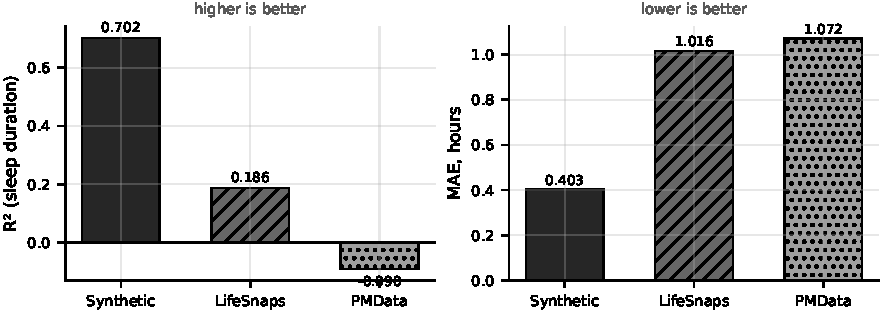
\includegraphics[width=\columnwidth]{fig2_synthetic_vs_real.pdf}
\caption{The synthetic-to-real gap. Identical model, features and protocol, only
the data changes.}
\label{fig:synthgap}
\end{figure}

Across splits $R^2$ ranges from $-0.077$ to $+0.395$, so no single-split figure
is reportable, though the interval still excludes zero on LifeSnaps.
\textbf{On PMData the duration model does not replicate}, at $R^2 = -0.090$,
which is worse than predicting the mean. We state that as a failed replication
rather than a smaller effect. The regularity classifier does replicate, at AUC
0.660 (95\% CI 0.610--0.710) on LifeSnaps against 0.675 on PMData, both
excluding chance.

We report this because training on simulated data is common when real cohorts
are unavailable, and because it is a limitation of our own work before it is a
finding about anyone else's. Design decisions we made against the simulation may
be tuned to a world more predictable than the real one.

\subsection{Calibrated, and weakly informative}

Over 3,180 held-out person-nights from 46 participants the stated reliability is
well calibrated, at an expected calibration error of 0.0148 (95\% CI
0.0139--0.0571). Calibration alone is insufficient and we report Brier alongside
for that reason, since a predictor that always returns the base rate attains a
perfect ECE of 0.0000 while carrying no information. Brier separates them, at
0.1727 (CI 0.1490--0.2003) against 0.1898 for the base-rate predictor.

The honest description is \textbf{well calibrated and weakly informative}, which
is the combination honest refusal requires. The model does not know much, but it
knows how much it knows. This is a claim about internal consistency rather than
external validity. When the system states 85\%, roughly 85\% of those instances
satisfy the stated criterion, which is exactly the property a refusal mechanism
needs, because refusal is an assertion about the model's own confidence rather
than about the world.

\subsection{Refusal beats promising, and forward prediction refuses best}

Table~\ref{tab:refusal} reports over-promise rate, meaning the rate of promising
a target the held-out participant's own achieved rate could not deliver. The
model-free baselines have no mechanism for declining (Fig.~\ref{fig:refusal}), so at a 0.95 target they
promise every instance and are wrong every time.

\begin{table}[t]
\caption{Over-promise rate by method and target (lower is better)}
\label{tab:refusal}
\centering
\small
\begin{tabular}{lcccc}
\toprule
Target & Always & Fixed & Inverse & Forward \\
 & promise & rule & (ours) & prediction \\
\midrule
0.70 & 0.376 & 0.376 & 0.372 & \textbf{0.294} \\
0.80 & 0.614 & 0.614 & 0.473 & \textbf{0.261} \\
0.90 & 0.867 & 0.867 & 0.068 & \textbf{0.016} \\
0.95 & 1.000 & 1.000 & 0.040 & \textbf{0.013} \\
\bottomrule
\end{tabular}
\end{table}

\begin{figure}[t]
\centering
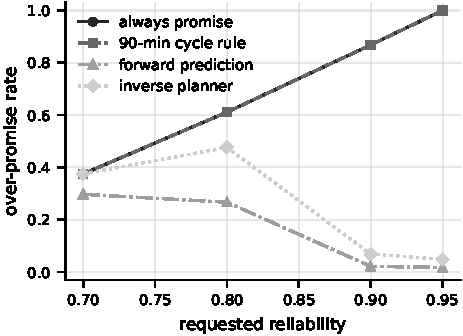
\includegraphics[width=\columnwidth]{fig4_refusal_quality.pdf}
\caption{Over-promise rate against requested reliability. The model-free
baselines diverge as the target rises because they have no mechanism for
declining, while both model-based methods fall away as refusal engages.}
\label{fig:refusal}
\end{figure}

\textbf{The informative comparison is forward prediction}, which uses the same
model and differs only in that it does not search, and it beats our method at
every target. We report this rather than omitting it, and we do not count it in
our favour, but it should not be read as evidence that inversion hurts. The two
make different kinds of promise. Forward prediction claims that the instance as
it already stands clears the target, and the observed outcome tests that claim
directly. Inversion claims that a \emph{changed} input would clear it, and no
participant adopted a changed input on our instruction, so the observed outcome
tests an instance the recommendation was not about. The comparison is between a
claim this dataset can check and one it cannot, and separating them requires
intervention rather than more observation.

%% ===============================================================
\section{Limitations}
\label{sec:limitations}

We state these before a reader has to find them.

\textbf{The target is constructed and does not track wellbeing.} Neither dataset
contains an alarm or an intended wake time, so the label measures deviation from
personal schedule and nothing more. Tested against self-reported sleep quality
($d = -0.093$), readiness ($-0.026$) and a tiredness indicator ($-0.041$), all
effects were negligible and two pointed the wrong way. We therefore renamed the
target from wake success to wake-time regularity, and we claim nothing about how
anyone felt.

\textbf{The models are weak in absolute terms.} $R^2$ 0.186 and AUC 0.660
explain a minority of variance. We argue this motivates rather than undermines
the contribution, since a method working from a signal this thin should decline
to promise, but a reader who wants strong point predictions will not find them
here.

\textbf{The simulation scenarios are ours.} Soundness holds across seven
ground-truth models we designed, including cases built to defeat greedy search.
They are principled rather than convenient, but they are not a proof, and a
different family of response surfaces might expose different behaviour.

\textbf{Part of the input space is unpopulated in public data.} Two of the four
out-of-horizon inputs are absent from every public wearable dataset, and four of
seven controllable inputs are absent from these cohorts, so the coordinate
ascent results are measured in simulation with the full control set and are an
upper bound on what that component contributes in deployment today.

\textbf{No deployment study.} The end-to-end claim, that following the advice
improves outcomes, is not established and cannot be from retrospective data. Our
within-participant matched analysis is directionally positive at every tolerance
and excludes zero at none of them, with only 9 to 11 participants contributing a
paired difference. Detecting an effect of the observed magnitude would need
roughly 50 to 75 participants.

\textbf{Cohort generalisability.} 85 participants across two cohorts, neither
demographically representative, and neither dataset yields a numeric age, so no
age-adjusted analysis is possible. Sleep staging is consumer-grade rather than
polysomnography, and its error is not independent of the behaviours we model.

%% ===============================================================
\section{Conclusion}
\label{sec:conclusion}

We treated a trained classifier as a constraint to solve against rather than a
forecast to read, and asked what a user must change to attain a reliability they
choose. Two things follow from that change of question. Inputs must be
partitioned by when the user can act on them rather than by whether they can act
at all, and that partition is not the actionable versus immutable split recourse
uses, because the most informative inputs are often changeable on a horizon
longer than the one being planned over. And infeasibility must be reported
rather than suppressed, because a method that cannot decline will promise
whatever its model happens to output.

The search is sound. Against exhaustive ground truth it never promised a target
it could not reach, returned the optimal admissible setting in every case, and
erred only by refusing three times when a plan existed. The ablation isolates
the horizon partition as the single component whose removal makes it unsound.
What we have not shown is that following the advice improves outcomes, which
requires giving people the recommendation and measuring what happens, and our
matched analysis is only large enough to size that study. The method is ready
for it. The claim is not yet earned.

\section*{Reproducibility}

All results regenerate from committed code with pinned versions and fixed seeds.
311 tests cover the pipeline, including assertions that participant splits are
disjoint, that outcome columns cannot become predictors, and that trailing
features use strictly prior nights. Datasets are not redistributed and both are
obtainable without application. Code and reproduction instructions are available
at an anonymised URL for review.\footnote{%%
\url{https://anonymous.4open.science/r/reliability-targeted-bedtime-planning-103C/}}

%% ===============================================================
\begin{thebibliography}{9}

\bibitem{wachter}
S. Wachter, B. Mittelstadt, and C. Russell, ``Counterfactual explanations
without opening the black box: automated decisions and the GDPR,''
\emph{Harvard Journal of Law \& Technology}, vol.~31, no.~2, pp.~841--887, 2018.

\bibitem{ustun}
B. Ustun, A. Spangher, and Y. Liu, ``Actionable recourse in linear
classification,'' in \emph{Proc. Conf. Fairness, Accountability, and
Transparency (FAT*)}, 2019, pp.~10--19.

\bibitem{dice}
R. K. Mothilal, A. Sharma, and C. Tan, ``Explaining machine learning classifiers
through diverse counterfactual explanations,'' in \emph{Proc. Conf. Fairness,
Accountability, and Transparency (FAT*)}, 2020, pp.~607--617.

\bibitem{smartalarm}
C. Campanella, K. Byun, A. Senerat, L. Li, R. Zhang, S. Aristizabal, P. Porter,
and B. Bauer, ``The efficacy of a multimodal bedroom-based `smart' alarm system
on mitigating the effects of sleep inertia,'' \emph{Clocks \& Sleep}, vol.~6,
no.~1, pp.~183--199, 2024.

\bibitem{sathya}
A. Sathyanarayana, S. Joty, L. Fernandez-Luque, F. Ofli, J. Srivastava,
A. Elmagarmid, T. Arora, and S. Taheri, ``Sleep quality prediction from wearable
data using deep learning,'' \emph{JMIR mHealth and uHealth}, vol.~4, no.~4,
art.~e125, 2016.

\bibitem{fellger}
A. Fellger, G. Sprint, D. Weeks, E. Crooks, and D. J. Cook, ``Wearable
device-independent next day activity and next night sleep prediction for
rehabilitation populations,'' \emph{IEEE Journal of Translational Engineering in
Health and Medicine}, vol.~8, art.~2700509, 2020.

\bibitem{lifesnaps}
S. Yfantidou, C. Karagianni, S. Efstathiou, A. Vakali, J. Palotti, D. P.
Giakatos, T. Marchioro, A. Kazlouski, E. Ferrari, and
\v{S}. Girdzijauskas, ``LifeSnaps, a 4-month multi-modal dataset capturing
unobtrusive snapshots of our lives in the wild,'' \emph{Scientific Data},
vol.~9, art.~663, 2022.

\bibitem{pmdata}
V. Thambawita, S. A. Hicks, H. Borgli, H. K. Stensland, D. Jha, \emph{et al.},
``PMData: a sports logging dataset,'' in \emph{Proc. 11th ACM Multimedia Systems
Conf.\ (MMSys)}, 2020, pp.~231--236.

\end{thebibliography}

\end{document}
